\documentclass[main.tex]{subfiles}

\begin{document}

\subsection{StarPU} \label{section:impl_starpu}

For the final implementation, using the \starpu framework, most of the remaining work consisted on reusing the existing code for each computational tasks, and submit them as tasks to be scheduled by \starpu. The development process of the previous implementations (\cpu and \cuda) resulted in a very modular solution, with very little coupling\footnote{The degree of dependency between the multiple modules of a system. Tight coupling tends to difficult refactoring of one module without requiring subsequent changes to dependant modules, difficulting code} between tasks implementation and the algorithm and scheduling code being used.

\subsubsection{Early Decisions}

An early decision for this implementation was to consider only the low-level API, and not the \texttt{pragma}-based one (see \cref{section:starpu_api}). The reason for this is due to the high-level version being an early product, still being in earlier development stages, and not being fully capable of providing the full set of features of \starpu.

Additionally, the actual documentation for the framework is almost entirely focused on the low-level functions, making it easier getting up to speed and understand its usage.

An additional decision that was enforced by the existing implementations is related to the used task scheduling policy. Since the \cpu implementation of all parallelizable tasks was based on \openmp, it was intuitive to approach the problem by using the capabilities of parallel tasks and combined workers of \starpu (see \cref{section:starpu_multithreading}). The only drawback that comes from this is that only the parallel-aware task schedulers (\texttt{pheft} and \texttt{peager}) are capable of parallelizing \cpu tasks. This means that when using a non-parallel-aware scheduler, \cpu tasks such as \textbf{Advance Photon Paths} will increase in cost.

\subsubsection{Data Management}

The first step for this implementation was to refactor data management, letting \starpu handle all necessary data for the algorithm. One exception was made to this, regarding the input information for the 3D scene. This information is stored in a somewhat complex structure, as opposed to all other dynamic data used throughout the photon mapping algorithm, which consists only on vectors whose size can be static and predetermined.

A small change was necessary in the lookup table build process. This task previously generated a dynamically sized structure, since it is dependent on the number of photons that intersect the scene within the current radius of each hit point, which cannot be predetermined.

One solution for this would be to only register the lookup table in a \starpu data handle only after its generation is complete, and the size can be determined. This is not a desirable solution, as it would introduce a barrier on that point of the iteration, and forcing all future tasks to be submitted only once the lookup table build process is complete. This would prevent \starpu from having knowledge on future tasks, and preventing it from asynchronously prepare data buffers to solve dependencies, increasing the latency caused by the imposed barrier.

This seems to be a rather harsh limitation of \starpu, as irregular sized structures are commonly used. However, an alternative solution is possible for this specific problem. The cell size used for the hash grid is based on the photon radius for the current iteration, in such a way that a cell will never have a width, height or depth greater than the current radius. With that any given hit point will always intersect at most 8 cells. Thus, it can be determined that the maximum hash table size can be set as $8 * \#hit\_points$, for any iteration.

Following this constraint, the hash table structure was refactored to be a fixed-size one, allowing \starpu to handle it without the need for barrier, and allowing future tasks to be submitted at will, using the lookup table data handle as a regular data buffer and dependency.

\subsubsection{Task Submission}

The other main change required is to wrap tasks around \starpu API calls. All data for each iteration is assigned to an individual data handle. No allocations are ever done manually during the main loop, making all memory managed by \starpu. While in the \cpu and \cuda version, only a single iteration is considered at a time, so task invocation is made synchronously, here all tasks are submitted asynchronously, and dependencies are implicitly given by the data handles required by each task. These dependencies are represented in \cref{fig:deps}.

\begin{figure}[!htp]
  \centering
  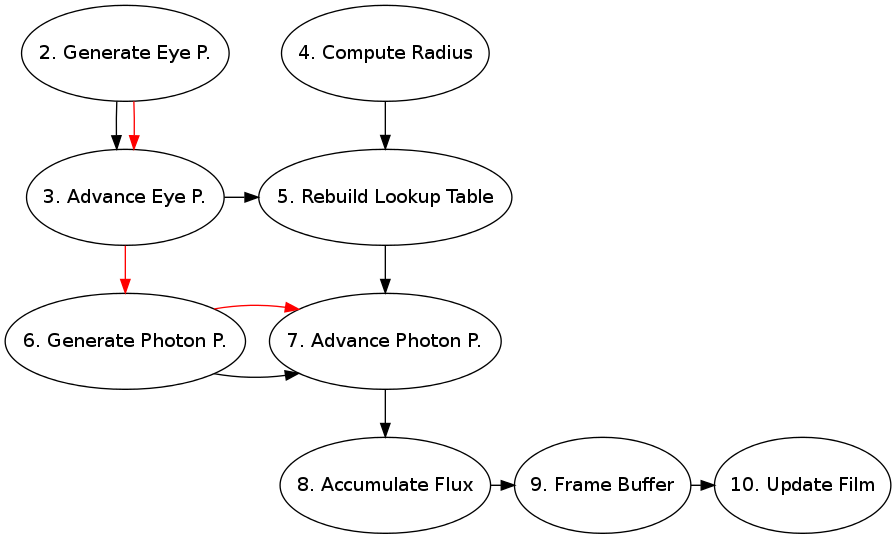
\includegraphics[width=0.8\textwidth]{deps.png}
  \caption[Dependency graph of an iteration of SPPMPA]{Dependency graph of an iteration of SPPMPA. Red arrows represent dependencies related to the seed buffer, which are not imposed on the algorithm itself, but only a limitation of the implementation \label{fig:deps}}
\end{figure}

It can be seen from the graph that some task concurrency is possible, although limited. It is expected that the most time consuming tasks are \textbf{Advance Eye Paths} and \textbf{Advance Photon Paths}, as they compute scene intersections. \textbf{Rebuild Lookup Table} can also be considered, especially when other tasks of the same iteration are run on a \gpu. This will require synchronization memory transactions to solve the dependencies of this task. Prefetching cannot be employed here by \starpu, as these dependencies are not available until the immediately previous tasks are computed. This could provide a large bottleneck for the performance of each individual iteration.

One of the limiting factors of these dependencies is related to the number generation method employed, which relies on a read-write seed buffer, with each new value requested updating the corresponding seed. As can be seen in the graph, only one relevant dependency is actually created by this, between \textbf{Advance Eye Paths} and \textbf{Generate Photon Paths}. These tasks should be considered independent, but share a dependency on the seed buffer, and thus cannot execute concurrently as it would be expected. Other dependencies are created from this limitation (shown in red in the graph), but they do not represent a problem, since their elimination would not introduce any new concurrency possibilities.

A solution for this would be to change the random number generation method, to one that would not require intermediate seed memory to be passed between each task. However, that was not attempted, as it would require additional effort in changing the algorithm, as well as the previous implementations (if coherence between them was to be kept), and choosing an adequate and efficient new method. The final solution actually came as a consequence of enabling concurrency between iterations, explained in the next section.


\subsubsection{Enabling Concurrent Iterations} \label{section:starpu_concurrent_iters}

Since the high amount of dependencies between tasks does not allow a good degree of concurrency within a single iteration, efforts were focused in allowing the execution of multiple iterations concurrently. This is one of the main reasons SPPMPA was the only one focused on, as other versions without the probabilistic radius estimation would introduce dependencies between each iteration, preventing their parallelization.

The initial approach to port the implementation to \starpu relied on data handles being declared at the start of the rendering process, and released at the end.

\begin{listing}[htp]
  \inputminted[linenos,tabsize=4]{c++}{code/starpu_initial.cpp}

  \caption{The beginning of the main rendering loop, with global data handles}
  \label{lst:starpu_initial}
\end{listing}

As shown in \cref{lst:starpu_initial}, data handles are created and kept during the whole rendering process. In practice, this means that each iteration will depend on the same data buffers as the previous one, even though they are to be completely re-written, and their previous values ignored. This is not desirable, as it prevents concurrency between iterations, just like it happens due to the seed buffer dependency previously explained.

An alternative solution is to declare the handles in-loop, as shown in \cref{lst:starpu_handles_in_loop}.

\begin{listing}[htp]
  \inputminted[linenos,tabsize=4]{c++}{code/starpu_handles_in_loop.cpp}

  \caption{The beginning of the main rendering loop, now with in-loop data handles}
  \label{lst:starpu_handles_in_loop}
\end{listing}

With this method, each iteration declares its own copy of the required data. \starpu provides the \texttt{starpu\_data\_unregister\_submit} API call, which instructs the library that the given data buffer can be discarded as soon as existing tasks depending on it are finished. Since data is local to each iteration, this can actually be considered a more intuitive way to approach the problem.

However, an additional problem arose from this approach. Due to the asynchronous nature of the tasks, the program actually submits every single iteration to the scheduler, meaning that multiple copies of the \texttt{eye\_paths} and \texttt{hit\_points} buffers will be immediately requested. For a large enough number of iterations, this resulted in memory problems, and eventually program failures. Since \starpu does not provide any method to control this, the limitation had to be imposed manually, by inserting a barrier every few iterations (with the actual number being a configurable value).

\end{document}
